\documentclass[20pt, a0paper, portrait]{tikzposter}

\title{\fontsize{45pt}{30pt}\selectfont Prédiction des validations journalières par gare chez SNCF-Transilien}
\author{Girondin Audric}
\date{\today}
\institute{Master 2 MIASHS, Université Montpellier III}

\usepackage[utf8]{inputenc}
\usepackage[french]{babel}
\usepackage{graphicx}
\usepackage{amsmath}
\usetheme{Rays}
\usepackage{lipsum}
\usepackage{tikz}
\usepackage{multirow}
\usepackage{array}
\usepackage{hyperref}


\begin{document}

\maketitle

% CONTEXTE ET OBJECTIF
\begin{columns}
    \column{0.5}
    \block{Contexte et objectif}{

Participation à un challenge data organisé par SNCF-Transilien. \url{https://challengedata.ens.fr/participants/challenges/149/} \\ 

\textbf{Contexte :} SNCF-Transilien est l'opérateur des trains de banlieue en Île-de-France, faisant circuler plus de 6 200 trains et transportant 3,2 millions de voyageurs quotidiennement. Ces voyageurs valident leurs cartes à puce sur les portiques en moyenne 2,3 millions de fois par jour. Entre 2015 et 2019, le nombre de validations a connu une croissance annuelle de 6\%. Anticiper cette évolution permettrait à SNCF-Transilien d'améliorer la performance de son exploitation et d'adapter son offre.\\

\textbf{Objectif :} Prédire à moyen-long terme le nombre de validations par jour et par gare pour anticiper les volumes de voyageurs, mieux comprendre les dynamiques d'affluence et accompagner les évolutions du réseau.
\\

\textbf{Métrique d'évaluation :} L’erreur est mesurée à l’aide du \textit{Mean Absolute Percentage Error (MAPE)} :
\[
\text{MAPE} = \frac{1}{n} \sum_{i=1}^{n} \left| \frac{y_i - \hat{y}_i}{y_i} \right|
\]

}

\column{0.5}
    \block{Description des données}{
        \textbf{Origine :} Données fournies par Île-de-France Mobilités.\\
        \textbf{Train.csv :} 1 237 971 lignes, 6 colonnes (2015--2022).\\
        \textbf{Test.csv :} 78 652 lignes, 5 colonnes (janvier--juin 2023).\\
        \textbf{Nombre de stations :} 448 gares distinctes.\\
        \textbf{Variables :}
        \begin{itemize}
            \item \texttt{date} : jour de la validation
            \item \texttt{station} : identifiant anonymisé de la gare
            \item \texttt{job, ferie, vacances} : indicateurs contextuels
            \item \texttt{y} : nombre de validations
        \end{itemize}

        \textbf{Features engineering :}
        \begin{itemize}
            \item Variables temporelles : \texttt{weekday}, \texttt{weekofyear}, \texttt{month}, \texttt{quarter}, etc.
            \item Lags : \texttt{lag\_1\_log}, \texttt{lag\_7\_log}, \texttt{lag\_30\_log}, \texttt{lag\_365\_log}
            \item Encodage des stations
            \item Log-transformation de \texttt{y}
        \end{itemize}
        \vspace{2.6cm}

    }

\end{columns}

% ANALYSE EXPLORATOIRE
\block{Analyse exploratoire des données}{
\begin{center}
\begin{minipage}[t]{0.48\linewidth}
    \centering
    \textbf{Évolution du nombre total de validations (y) de 2015 à 2022}\\
    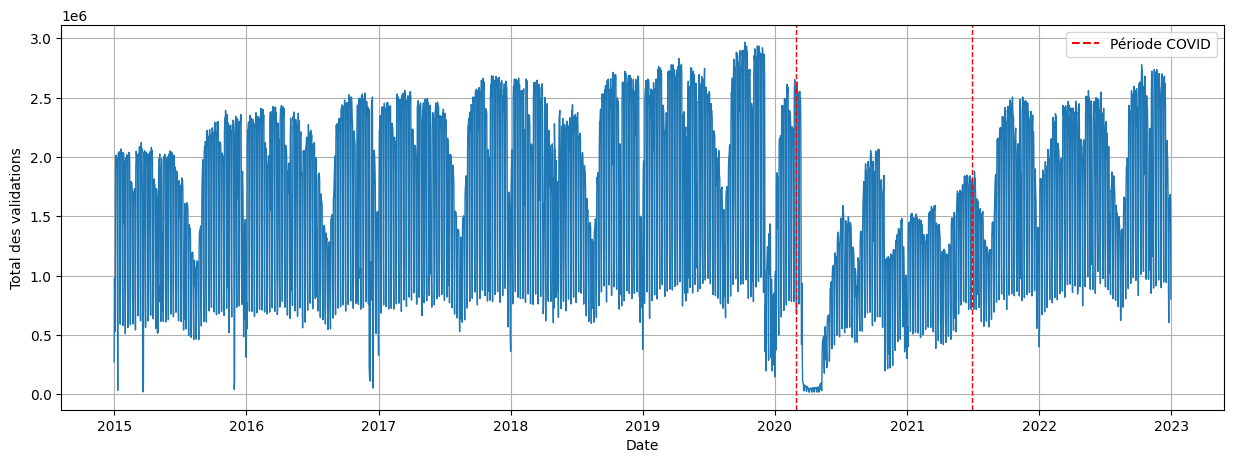
\includegraphics[width=35cm, height=9cm]{images/evo.png}

    \vspace{0.1em}
    \begin{itemize}
        \item Tendance haussière de 2015 à 2019.
        \item Saisonnalité annuelle très forte.
        \item Chute brutale en 2020 puis reprise progressive (effet COVID-19).
        \item Régularité retrouvée à partir de 2022, mais un niveau encore légèrement inférieur à 2019.
    \end{itemize}
\end{minipage}
\hfill
\begin{minipage}[t]{0.5\linewidth}
    \centering
    \textbf{Autocorrélation des validations (y)}\\
    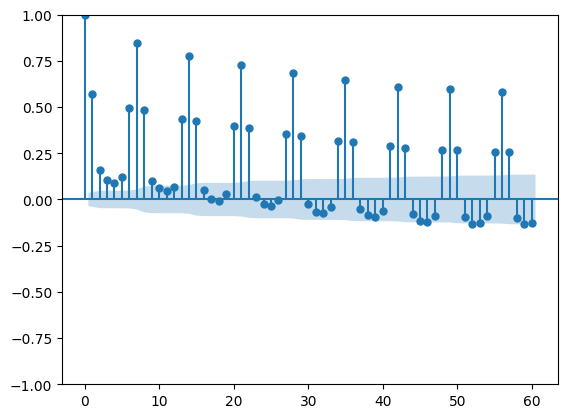
\includegraphics[width=33cm, height=9cm]{images/auto.png}

    \vspace{0.1em}
    \begin{itemize}
        \item Saisonnalité hebdomadaire très marquée : des pics nets tous les 7 jours (trafic récurrent les mêmes jours de semaine).
        \item Autocorrélation qui décroît lentement indique une tendance à long terme, en plus de la saisonnalité.
        \item Série très autocorrélée jusqu’à 60 jours (corrélation significative).
    \end{itemize}
\end{minipage}
\end{center}
}

\begin{columns}
    \column{0.5}
    \block{Méthodologie}{
        \textbf{Approches classiques (sans Machine Learning) :}

\medskip
            \begin{itemize}
                \bigskip
                \item \textbf{Benchmark} : recopie de 2022 sur 2023 en alignant les jours
                \item Projection de tendance de 2021--2022 sur 2023
            \end{itemize}

        \bigskip
       
        \textbf{Prétraitements et stratégies de modélisation :}

    

\begin{itemize}

    \bigskip

    \item Trois stratégies testées pour traiter la période COVID :
    \bigskip

        \textbullet\ Ajout d’une variable indicatrice COVID\\
         \textbullet\ Remplacement des données par lissage ou moyenne des y précédents\\
         \textbullet\ Entraînement uniquement sur la période post-COVID (2021+)

    \bigskip
    \item Autres approches explorées :
    
    \bigskip

         \textbullet\ SARIMA par station\\
         \textbullet\ XGBoost par station
\end{itemize}

        \bigskip

            \textbf{Modèles Machine Learning et Deep Learning :}

            \bigskip

            \begin{itemize}
                \item {Prophet}
                \item {ARIMA}
                \item {XGBoost}
                \item {LightGBM}
                \item {Réseaux de neurones} : CNN, LSTM, GRU
                \item {Transformers} pour séries temporelles multivariées
            \end{itemize}
            \vspace{1cm}

    }

    \column{0.5}
    \block{Résultats}{
    \textbf{Sélection de modèles sur jeu de validation (minimisation de la MAPE) }
        \begin{center}
            \begin{tabular}{|l|l|c|}
            \hline
            \textbf{Stratégies} & \textbf{Meilleurs Modèles} & \textbf{MAPE} \\
            \hline
            \multirow{2}{*}{Variable COVID} 
                & LightGBM                & 0.77 \\
                & XGBoost               & 0.75\\
            \hline
            \multirow{2}{*}{Remplacement des données}
                & LSTM                & 1.52\\
                & CNN               & 1.00 \\
            \hline
            \multirow{2}{*}{Apprentissage post-COVID (2021+)} 
                & LightGBM                & pas assez de données pour évaluer \\
                & XGBoost               & pas assez de données pour évaluer \\
            \hline
                \textbf{XGBoost par station} & \textbf{XGBoost} & \textbf{0.31} \\
            \hline
                
            \end{tabular}
            \end{center}
        
    \textbf{Classement des soumissions par score public (MAPE)}
        \begin{center}
            \begin{tabular}{|c|l|l|c|}
                \hline
                \textbf{Rang} & \textbf{Méthode} & \textbf{Features} & \textbf{Score} \\
                \hline
                1 & \textbf{XGBoost par station post-COVID} & \textbf{Features engineering + indicateurs contextuels} & \textbf{143,64} \\
                2 & {XGBoost par station} & {Features engineering et indicateurs contextuels} & {150.22} \\
                3 & XGBoost par station & Indicateurs contextuels & 182.66 \\
                4 & XGBoost post-COVID & Features engineering et indicateurs contextuels & 217.43 \\
                5 & SARIMA & Features engineering et indicateurs contextuels & 231.04 \\
                6 & LightGBM post-COVID & Features engineering et indicateurs contextuels & 252.35 \\
                7& Projection des tendances 2021-2022 & Copie 2022 + $\Delta (2021-2022)$  & 349,52 \\
                \hline
                \end{tabular}
        \end{center}

    \begin{itemize}
        \item \textbf{Score du Benchmark officiel du challenge :} 177,0825 (91\textsuperscript{e} place)
        \item \textbf{Mon classement :} 66\textsuperscript{e} sur 200 participants
    \end{itemize}
    }
\end{columns}


\block{Analyse des résidus}{
\begin{columns}
    \column{0.5}
    \raggedright
    \textbf{Observations clés :}
    \bigskip
    \begin{itemize}
        \item Les erreurs sont plus élevées pour les faibles valeurs prédites → instabilité à bas trafic (effet d’hétéroscédasticité).
        \item Pour les fortes affluences (\(\geq 100\,000\)), les résidus sont resserrés autour de zéro : meilleure précision.
        \item Les erreurs sont globalement symétriques autour de 0 mais présence d'outliers.
    \end{itemize}

    \vspace{2cm}
    \textbf{Perspectives:}
    \bigskip
    \begin{itemize}
        \item Clustering des gares pour créer des modèles spécialisés
        \item Ajouter des variables extérieures : événements, météo, etc.
        \item Analyser les outliers pour mieux comprendre les erreurs
        \item Tester des modèles hybrides (ex. LSTM + XGBoost)
    \end{itemize}

    \column{0.5}
    \vspace*{-16em}
    \hspace*{42cm}
    \textbf{Graphique des résidus sur le jeu de validation du meilleur modèle (XGBoost par station avec features)}

    \vspace{0.5em}
    \hspace*{40cm}
    \includegraphics[width=35cm, height=11cm]{images/résidus.png}

\end{columns}
}

% REFERENCES
    \block{Références}{
        \begin{itemize}
            \item Olah, C. (2015). \textit{Understanding LSTM Networks}. arXiv:1406.1078v3 [cs.CL].
            \item Siami-Namini, S., Siami-Namin, A. (2018). \textit{Forecasting Economic and Financial Time Series: ARIMA vs. LSTM}. Texas Tech University.
            \item Taylor, S.J., Letham, B. (2017). \textit{Forecasting at Scale}. Facebook.
            \item Vaswani, A., et al. (2017). \textit{Attention Is All You Need}. arXiv:1706.03762v7 [cs.CL].
            \item Chen, T., Guestrin, C. (2016). \textit{XGBoost: A Scalable Tree Boosting System}. arXiv:1603.02754v3 [cs.LG].
        \end{itemize}
        }

\end{document}